\documentclass[tikz]{standalone}

\usepackage[T1]{fontenc}
\usepackage[utf8]{inputenc}
\usepackage{eulervm}
\usepackage{amsmath}
\usepackage{bm}
\usepackage{tikz}
\usepackage{environ}

\usetikzlibrary{fit}
\usetikzlibrary{patterns}
\usetikzlibrary{arrows}

\usepackage{color}

\definecolor{Comment}{RGB}{97,161,176}

\definecolor{btfGreen}{RGB}{51,160,44}
\definecolor{btfRed}{RGB}{190,60,90}

\definecolor{bleuUni}{RGB}{0, 157, 224}
\definecolor{marronUni}{RGB}{68, 58, 49}
\definecolor{grayMarronUni}{RGB}{60, 60, 60}
\definecolor{grayBleuUni}{RGB}{118, 118, 118}

\definecolor{bluecite}{HTML}{009DE0}

\definecolor{Paired-2}{RGB}{166,206,227}
\definecolor{Paired-1}{RGB}{31,120,180}
\definecolor{Paired-4}{RGB}{178,223,138}
\definecolor{Paired-3}{RGB}{51,160,44}
\definecolor{Paired-6}{RGB}{251,154,153}
\definecolor{Paired-5}{RGB}{227,26,28}
\definecolor{Paired-8}{RGB}{253,191,111}
\definecolor{Paired-7}{RGB}{255,127,0}
\definecolor{Paired-10}{RGB}{202,178,214}
\definecolor{Paired-9}{RGB}{106,61,154}
\definecolor{Paired-12}{RGB}{255,255,153}
\definecolor{Paired-11}{RGB}{177,89,40}
\definecolor{Accent-1}{RGB}{127,201,127}
\definecolor{Accent-2}{RGB}{190,174,212}
\definecolor{Accent-3}{RGB}{253,192,134}
\definecolor{Accent-4}{RGB}{255,255,153}
\definecolor{Accent-5}{RGB}{56,108,176}
\definecolor{Accent-6}{RGB}{240,2,127}
\definecolor{Accent-7}{RGB}{191,91,23}
\definecolor{Accent-8}{RGB}{102,102,102}
\definecolor{Spectral-1}{RGB}{158,1,66}
\definecolor{Spectral-2}{RGB}{213,62,79}
\definecolor{Spectral-3}{RGB}{244,109,67}
\definecolor{Spectral-4}{RGB}{253,174,97}
\definecolor{Spectral-5}{RGB}{254,224,139}
\definecolor{Spectral-6}{RGB}{255,255,191}
\definecolor{Spectral-7}{RGB}{230,245,152}
\definecolor{Spectral-8}{RGB}{171,221,164}
\definecolor{Spectral-9}{RGB}{102,194,165}
\definecolor{Spectral-10}{RGB}{50,136,189}
\definecolor{Spectral-11}{RGB}{94,79,162}
\definecolor{Set1-1}{RGB}{228,26,28}
\definecolor{Set1-2}{RGB}{55,126,184}
\definecolor{Set1-3}{RGB}{77,175,74}
\definecolor{Set1-4}{RGB}{152,78,163}
\definecolor{Set1-5}{RGB}{255,127,0}
\definecolor{Set1-6}{RGB}{255,255,51}
\definecolor{Set1-7}{RGB}{166,86,40}
\definecolor{Set1-8}{RGB}{247,129,191}
\definecolor{Set1-9}{RGB}{153,153,153}
\definecolor{Set2-1}{RGB}{102,194,165}
\definecolor{Set2-2}{RGB}{252,141,98}
\definecolor{Set2-3}{RGB}{141,160,203}
\definecolor{Set2-4}{RGB}{231,138,195}
\definecolor{Set2-5}{RGB}{166,216,84}
\definecolor{Set2-6}{RGB}{255,217,47}
\definecolor{Set2-7}{RGB}{229,196,148}
\definecolor{Set2-8}{RGB}{179,179,179}
\definecolor{Dark2-1}{RGB}{27,158,119}
\definecolor{Dark2-2}{RGB}{217,95,2}
\definecolor{Dark2-3}{RGB}{117,112,179}
\definecolor{Dark2-4}{RGB}{231,41,138}
\definecolor{Dark2-5}{RGB}{102,166,30}
\definecolor{Dark2-6}{RGB}{230,171,2}
\definecolor{Dark2-7}{RGB}{166,118,29}
\definecolor{Dark2-8}{RGB}{102,102,102}
\definecolor{Reds-1}{RGB}{255,245,240}
\definecolor{Reds-2}{RGB}{254,224,210}
\definecolor{Reds-3}{RGB}{252,187,161}
\definecolor{Reds-4}{RGB}{252,146,114}
\definecolor{Reds-5}{RGB}{251,106,74}
\definecolor{Reds-6}{RGB}{239,59,44}
\definecolor{Reds-7}{RGB}{203,24,29}
\definecolor{Reds-8}{RGB}{165,15,21}
\definecolor{Reds-9}{RGB}{103,0,13}
\definecolor{Greens-1}{RGB}{247,252,245}
\definecolor{Greens-2}{RGB}{229,245,224}
\definecolor{Greens-3}{RGB}{199,233,192}
\definecolor{Greens-4}{RGB}{161,217,155}
\definecolor{Greens-5}{RGB}{116,196,118}
\definecolor{Greens-6}{RGB}{65,171,93}
\definecolor{Greens-7}{RGB}{35,139,69}
\definecolor{Greens-8}{RGB}{0,109,44}
\definecolor{Greens-9}{RGB}{0,68,27}
\definecolor{Blues-1}{RGB}{247,251,255}
\definecolor{Blues-2}{RGB}{222,235,247}
\definecolor{Blues-3}{RGB}{198,219,239}
\definecolor{Blues-4}{RGB}{158,202,225}
\definecolor{Blues-5}{RGB}{107,174,214}
\definecolor{Blues-6}{RGB}{66,146,198}
\definecolor{Blues-7}{RGB}{33,113,181}
\definecolor{Blues-8}{RGB}{8,81,156}
\definecolor{Blues-9}{RGB}{8,48,107}


\begin{document}
  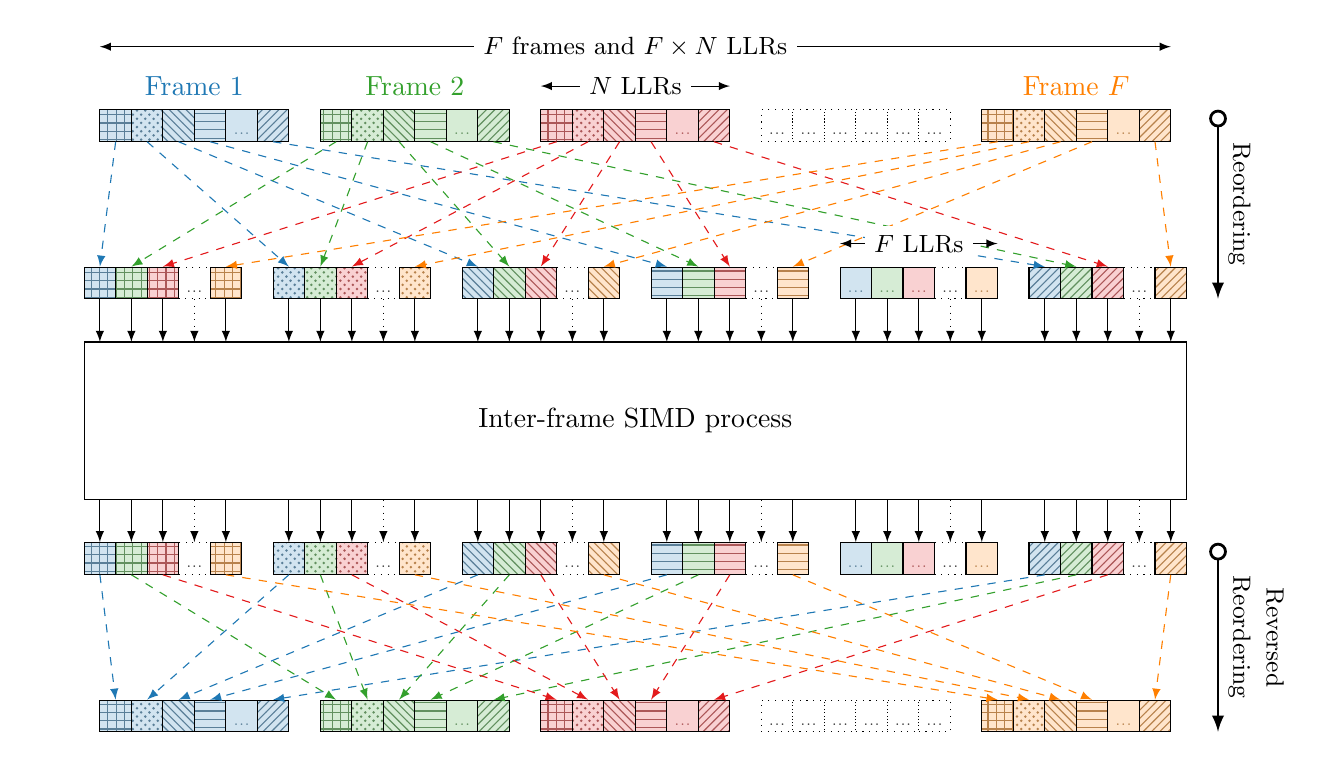
\begin{tikzpicture}
    \tikzset{ e1_f1/.style ={draw=black, minimum width=0.4cm, minimum height=0.4cm, text=black, preaction={fill=Paired-1!20}, pattern=grid,             pattern color=black!40!Paired-1!70} }
    \tikzset{ e2_f1/.style ={draw=black, minimum width=0.4cm, minimum height=0.4cm, text=black, preaction={fill=Paired-1!20}, pattern=crosshatch dots,  pattern color=black!40!Paired-1!70} }
    \tikzset{ e3_f1/.style ={draw=black, minimum width=0.4cm, minimum height=0.4cm, text=black, preaction={fill=Paired-1!20}, pattern=north west lines, pattern color=black!40!Paired-1!70} }
    \tikzset{ e4_f1/.style ={draw=black, minimum width=0.4cm, minimum height=0.4cm, text=black, preaction={fill=Paired-1!20}, pattern=horizontal lines, pattern color=black!40!Paired-1!70} }
    \tikzset{ ex_f1/.style ={draw=black, minimum width=0.4cm, minimum height=0.4cm, text=black, fill=Paired-1!20, label={[black!40!Paired-1!70,yshift=-0.45cm]above:\tiny{...}}           } }
    \tikzset{ en_f1/.style ={draw=black, minimum width=0.4cm, minimum height=0.4cm, text=black, preaction={fill=Paired-1!20}, pattern=north east lines, pattern color=black!40!Paired-1!70} }

    \tikzset{ e1_f2/.style ={draw=black, minimum width=0.4cm, minimum height=0.4cm, text=black, preaction={fill=Paired-3!20}, pattern=grid,             pattern color=black!40!Paired-3!70} }
    \tikzset{ e2_f2/.style ={draw=black, minimum width=0.4cm, minimum height=0.4cm, text=black, preaction={fill=Paired-3!20}, pattern=crosshatch dots,  pattern color=black!40!Paired-3!70} }
    \tikzset{ e3_f2/.style ={draw=black, minimum width=0.4cm, minimum height=0.4cm, text=black, preaction={fill=Paired-3!20}, pattern=north west lines, pattern color=black!40!Paired-3!70} }
    \tikzset{ e4_f2/.style ={draw=black, minimum width=0.4cm, minimum height=0.4cm, text=black, preaction={fill=Paired-3!20}, pattern=horizontal lines, pattern color=black!40!Paired-3!70} }
    \tikzset{ ex_f2/.style ={draw=black, minimum width=0.4cm, minimum height=0.4cm, text=black, fill=Paired-3!20, label={[black!40!Paired-3!70,yshift=-0.45cm]above:\tiny{...}}           } }
    \tikzset{ en_f2/.style ={draw=black, minimum width=0.4cm, minimum height=0.4cm, text=black, preaction={fill=Paired-3!20}, pattern=north east lines, pattern color=black!40!Paired-3!70} }

    \tikzset{ e1_f3/.style ={draw=black, minimum width=0.4cm, minimum height=0.4cm, text=black, preaction={fill=Paired-5!20}, pattern=grid,             pattern color=black!40!Paired-5!70} }
    \tikzset{ e2_f3/.style ={draw=black, minimum width=0.4cm, minimum height=0.4cm, text=black, preaction={fill=Paired-5!20}, pattern=crosshatch dots,  pattern color=black!40!Paired-5!70} }
    \tikzset{ e3_f3/.style ={draw=black, minimum width=0.4cm, minimum height=0.4cm, text=black, preaction={fill=Paired-5!20}, pattern=north west lines, pattern color=black!40!Paired-5!70} }
    \tikzset{ e4_f3/.style ={draw=black, minimum width=0.4cm, minimum height=0.4cm, text=black, preaction={fill=Paired-5!20}, pattern=horizontal lines, pattern color=black!40!Paired-5!70} }
    \tikzset{ ex_f3/.style ={draw=black, minimum width=0.4cm, minimum height=0.4cm, text=black, fill=Paired-5!20, label={[black!40!Paired-5!70,yshift=-0.45cm]above:\tiny{...}}           } }
    \tikzset{ en_f3/.style ={draw=black, minimum width=0.4cm, minimum height=0.4cm, text=black, preaction={fill=Paired-5!20}, pattern=north east lines, pattern color=black!40!Paired-5!70} }

    \tikzset{ e1_fy/.style ={draw=black, dotted, minimum width=0.4cm, minimum height=0.4cm, text=black, label={[black!80,yshift=-0.45cm]above:\tiny{...}}} }
    \tikzset{ e2_fy/.style ={draw=black, dotted, minimum width=0.4cm, minimum height=0.4cm, text=black, label={[black!80,yshift=-0.45cm]above:\tiny{...}}} }
    \tikzset{ e3_fy/.style ={draw=black, dotted, minimum width=0.4cm, minimum height=0.4cm, text=black, label={[black!80,yshift=-0.45cm]above:\tiny{...}}} }
    \tikzset{ e4_fy/.style ={draw=black, dotted, minimum width=0.4cm, minimum height=0.4cm, text=black, label={[black!80,yshift=-0.45cm]above:\tiny{...}}} }
    \tikzset{ ex_fy/.style ={draw=black, dotted, minimum width=0.4cm, minimum height=0.4cm, text=black, label={[black!80,yshift=-0.45cm]above:\tiny{...}}} }
    \tikzset{ en_fy/.style ={draw=black, dotted, minimum width=0.4cm, minimum height=0.4cm, text=black, label={[black!80,yshift=-0.45cm]above:\tiny{...}}} }

    \tikzset{ e1_ff/.style ={draw=black, minimum width=0.4cm, minimum height=0.4cm, text=black, preaction={fill=Paired-7!20}, pattern=grid,             pattern color=black!40!Paired-7!70} }
    \tikzset{ e2_ff/.style ={draw=black, minimum width=0.4cm, minimum height=0.4cm, text=black, preaction={fill=Paired-7!20}, pattern=crosshatch dots,  pattern color=black!40!Paired-7!70} }
    \tikzset{ e3_ff/.style ={draw=black, minimum width=0.4cm, minimum height=0.4cm, text=black, preaction={fill=Paired-7!20}, pattern=north west lines, pattern color=black!40!Paired-7!70} }
    \tikzset{ e4_ff/.style ={draw=black, minimum width=0.4cm, minimum height=0.4cm, text=black, preaction={fill=Paired-7!20}, pattern=horizontal lines, pattern color=black!40!Paired-7!70} }
    \tikzset{ ex_ff/.style ={draw=black, minimum width=0.4cm, minimum height=0.4cm, text=black, fill=Paired-7!20, label={[black!40!Paired-7!70,yshift=-0.45cm]above:\tiny{...}}           } }
    \tikzset{ en_ff/.style ={draw=black, minimum width=0.4cm, minimum height=0.4cm, text=black, preaction={fill=Paired-7!20}, pattern=north east lines, pattern color=black!40!Paired-7!70} }

    % input
    \node[e1_f1] (in_e1_f1) at ( 0.0, 3.75) {};
    \node[e2_f1] (in_e2_f1) at ( 0.4, 3.75) {};
    \node[e3_f1] (in_e3_f1) at ( 0.8, 3.75) {};
    \node[e4_f1] (in_e4_f1) at ( 1.2, 3.75) {};
    \node[ex_f1] (in_ex_f1) at ( 1.6, 3.75) {};
    \node[en_f1] (in_en_f1) at ( 2.0, 3.75) {};

    \node[e1_f2] (in_e1_f2) at ( 2.8, 3.75) {};
    \node[e2_f2] (in_e2_f2) at ( 3.2, 3.75) {};
    \node[e3_f2] (in_e3_f2) at ( 3.6, 3.75) {};
    \node[e4_f2] (in_e4_f2) at ( 4.0, 3.75) {};
    \node[ex_f2] (in_ex_f2) at ( 4.4, 3.75) {};
    \node[en_f2] (in_en_f2) at ( 4.8, 3.75) {};

    \node[e1_f3] (in_e1_f3) at ( 5.6, 3.75) {};
    \node[e2_f3] (in_e2_f3) at ( 6.0, 3.75) {};
    \node[e3_f3] (in_e3_f3) at ( 6.4, 3.75) {};
    \node[e4_f3] (in_e4_f3) at ( 6.8, 3.75) {};
    \node[ex_f3] (in_ex_f3) at ( 7.2, 3.75) {};
    \node[en_f3] (in_en_f3) at ( 7.6, 3.75) {};

    \node[e1_fy] (in_e1_fy) at ( 8.4, 3.75) {};
    \node[e2_fy] (in_e2_fy) at ( 8.8, 3.75) {};
    \node[e3_fy] (in_e3_fy) at ( 9.2, 3.75) {};
    \node[e4_fy] (in_e4_fy) at ( 9.6, 3.75) {};
    \node[ex_fy] (in_ex_fy) at (10.0, 3.75) {};
    \node[en_fy] (in_en_fy) at (10.4, 3.75) {};

    \node[e1_ff] (in_e1_ff) at (11.2, 3.75) {};
    \node[e2_ff] (in_e2_ff) at (11.6, 3.75) {};
    \node[e3_ff] (in_e3_ff) at (12.0, 3.75) {};
    \node[e4_ff] (in_e4_ff) at (12.4, 3.75) {};
    \node[ex_ff] (in_ex_ff) at (12.8, 3.75) {};
    \node[en_ff] (in_en_ff) at (13.2, 3.75) {};

    % reordered input
    \node[e1_f1] (rei_e1_f1) at (-0.2, 1.75) {};
    \node[e1_f2] (rei_e1_f2) at ( 0.2, 1.75) {};
    \node[e1_f3] (rei_e1_f3) at ( 0.6, 1.75) {};
    \node[e1_fy] (rei_e1_fy) at ( 1.0, 1.75) {};
    \node[e1_ff] (rei_e1_ff) at ( 1.4, 1.75) {};

    \node[e2_f1] (rei_e2_f1) at ( 2.2, 1.75) {};
    \node[e2_f2] (rei_e2_f2) at ( 2.6, 1.75) {};
    \node[e2_f3] (rei_e2_f3) at ( 3.0, 1.75) {};
    \node[e2_fy] (rei_e2_fy) at ( 3.4, 1.75) {};
    \node[e2_ff] (rei_e2_ff) at ( 3.8, 1.75) {};

    \node[e3_f1] (rei_e3_f1) at ( 4.6, 1.75) {};
    \node[e3_f2] (rei_e3_f2) at ( 5.0, 1.75) {};
    \node[e3_f3] (rei_e3_f3) at ( 5.4, 1.75) {};
    \node[e3_fy] (rei_e3_fy) at ( 5.8, 1.75) {};
    \node[e3_ff] (rei_e3_ff) at ( 6.2, 1.75) {};

    \node[e4_f1] (rei_e4_f1) at ( 7.0, 1.75) {};
    \node[e4_f2] (rei_e4_f2) at ( 7.4, 1.75) {};
    \node[e4_f3] (rei_e4_f3) at ( 7.8, 1.75) {};
    \node[e4_fy] (rei_e4_fy) at ( 8.2, 1.75) {};
    \node[e4_ff] (rei_e4_ff) at ( 8.6, 1.75) {};

    \node[ex_f1] (rei_ex_f1) at ( 9.4, 1.75) {};
    \node[ex_f2] (rei_ex_f2) at ( 9.8, 1.75) {};
    \node[ex_f3] (rei_ex_f3) at (10.2, 1.75) {};
    \node[ex_fy] (rei_ex_fy) at (10.6, 1.75) {};
    \node[ex_ff] (rei_ex_ff) at (11.0, 1.75) {};

    \node[en_f1] (rei_en_f1) at (11.8, 1.75) {};
    \node[en_f2] (rei_en_f2) at (12.2, 1.75) {};
    \node[en_f3] (rei_en_f3) at (12.6, 1.75) {};
    \node[en_fy] (rei_en_fy) at (13.0, 1.75) {};
    \node[en_ff] (rei_en_ff) at (13.4, 1.75) {};

    % connexions input -> reordered
    \draw[->,>=latex, dashed, Paired-1] (in_e1_f1.south) -- (rei_e1_f1.north);
    \draw[->,>=latex, dashed, Paired-1] (in_e2_f1.south) -- (rei_e2_f1.north);
    \draw[->,>=latex, dashed, Paired-1] (in_e3_f1.south) -- (rei_e3_f1.north);
    \draw[->,>=latex, dashed, Paired-1] (in_e4_f1.south) -- (rei_e4_f1.north);
    % \draw[->,>=latex, dashed, Paired-1] (in_ex_f1.south) -- (rei_ex_f1.north);
    \draw[->,>=latex, dashed, Paired-1] (in_en_f1.south) -- (rei_en_f1.north);

    \draw[->,>=latex, dashed, Paired-3] (in_e1_f2.south) -- (rei_e1_f2.north);
    \draw[->,>=latex, dashed, Paired-3] (in_e2_f2.south) -- (rei_e2_f2.north);
    \draw[->,>=latex, dashed, Paired-3] (in_e3_f2.south) -- (rei_e3_f2.north);
    \draw[->,>=latex, dashed, Paired-3] (in_e4_f2.south) -- (rei_e4_f2.north);
    % \draw[->,>=latex, dashed, Paired-3] (in_ex_f2.south) -- (rei_ex_f2.north);
    \draw[->,>=latex, dashed, Paired-3] (in_en_f2.south) -- (rei_en_f2.north);

    \draw[->,>=latex, dashed, Paired-5] (in_e1_f3.south) -- (rei_e1_f3.north);
    \draw[->,>=latex, dashed, Paired-5] (in_e2_f3.south) -- (rei_e2_f3.north);
    \draw[->,>=latex, dashed, Paired-5] (in_e3_f3.south) -- (rei_e3_f3.north);
    \draw[->,>=latex, dashed, Paired-5] (in_e4_f3.south) -- (rei_e4_f3.north);
    % \draw[->,>=latex, dashed, Paired-5] (in_ex_f3.south) -- (rei_ex_f3.north);
    \draw[->,>=latex, dashed, Paired-5] (in_en_f3.south) -- (rei_en_f3.north);

    \draw[->,>=latex, dashed, Paired-7] (in_e1_ff.south) -- (rei_e1_ff.north);
    \draw[->,>=latex, dashed, Paired-7] (in_e2_ff.south) -- (rei_e2_ff.north);
    \draw[->,>=latex, dashed, Paired-7] (in_e3_ff.south) -- (rei_e3_ff.north);
    \draw[->,>=latex, dashed, Paired-7] (in_e4_ff.south) -- (rei_e4_ff.north);
    % \draw[->,>=latex, dashed, Paired-7] (in_ex_ff.south) -- (rei_ex_ff.north);
    \draw[->,>=latex, dashed, Paired-7] (in_en_ff.south) -- (rei_en_ff.north);

    % inter-frame processing
    \node[draw=black, minimum width=14.0cm, minimum height=2.0cm] (inter_proc) at (6.6, 0.0) {Inter-frame SIMD process};

    % connexions input reordered -> process
    \draw[->,>=latex        ] (rei_e1_f1.south) -- (-0.2, 1.0);
    \draw[->,>=latex        ] (rei_e1_f2.south) -- ( 0.2, 1.0);
    \draw[->,>=latex        ] (rei_e1_f3.south) -- ( 0.6, 1.0);
    \draw[->,>=latex, dotted] (rei_e1_fy.south) -- ( 1.0, 1.0);
    \draw[->,>=latex        ] (rei_e1_ff.south) -- ( 1.4, 1.0);

    \draw[->,>=latex        ] (rei_e2_f1.south) -- ( 2.2, 1.0);
    \draw[->,>=latex        ] (rei_e2_f2.south) -- ( 2.6, 1.0);
    \draw[->,>=latex        ] (rei_e2_f3.south) -- ( 3.0, 1.0);
    \draw[->,>=latex, dotted] (rei_e2_fy.south) -- ( 3.4, 1.0);
    \draw[->,>=latex        ] (rei_e2_ff.south) -- ( 3.8, 1.0);

    \draw[->,>=latex        ] (rei_e3_f1.south) -- ( 4.6, 1.0);
    \draw[->,>=latex        ] (rei_e3_f2.south) -- ( 5.0, 1.0);
    \draw[->,>=latex        ] (rei_e3_f3.south) -- ( 5.4, 1.0);
    \draw[->,>=latex, dotted] (rei_e3_fy.south) -- ( 5.8, 1.0);
    \draw[->,>=latex        ] (rei_e3_ff.south) -- ( 6.2, 1.0);

    \draw[->,>=latex        ] (rei_e4_f1.south) -- ( 7.0, 1.0);
    \draw[->,>=latex        ] (rei_e4_f2.south) -- ( 7.4, 1.0);
    \draw[->,>=latex        ] (rei_e4_f3.south) -- ( 7.8, 1.0);
    \draw[->,>=latex, dotted] (rei_e4_fy.south) -- ( 8.2, 1.0);
    \draw[->,>=latex        ] (rei_e4_ff.south) -- ( 8.6, 1.0);

    \draw[->,>=latex        ] (rei_ex_f1.south) -- ( 9.4, 1.0);
    \draw[->,>=latex        ] (rei_ex_f2.south) -- ( 9.8, 1.0);
    \draw[->,>=latex        ] (rei_ex_f3.south) -- (10.2, 1.0);
    \draw[->,>=latex, dotted] (rei_ex_fy.south) -- (10.6, 1.0);
    \draw[->,>=latex        ] (rei_ex_ff.south) -- (11.0, 1.0);

    \draw[->,>=latex        ] (rei_en_f1.south) -- (11.8, 1.0);
    \draw[->,>=latex        ] (rei_en_f2.south) -- (12.2, 1.0);
    \draw[->,>=latex        ] (rei_en_f3.south) -- (12.6, 1.0);
    \draw[->,>=latex, dotted] (rei_en_fy.south) -- (13.0, 1.0);
    \draw[->,>=latex        ] (rei_en_ff.south) -- (13.4, 1.0);

    % reordered output
    \node[e1_f1] (reo_e1_f1) at (-0.2, -1.75) {};
    \node[e1_f2] (reo_e1_f2) at ( 0.2, -1.75) {};
    \node[e1_f3] (reo_e1_f3) at ( 0.6, -1.75) {};
    \node[e1_fy] (reo_e1_fy) at ( 1.0, -1.75) {};
    \node[e1_ff] (reo_e1_ff) at ( 1.4, -1.75) {};

    \node[e2_f1] (reo_e2_f1) at ( 2.2, -1.75) {};
    \node[e2_f2] (reo_e2_f2) at ( 2.6, -1.75) {};
    \node[e2_f3] (reo_e2_f3) at ( 3.0, -1.75) {};
    \node[e2_fy] (reo_e2_fy) at ( 3.4, -1.75) {};
    \node[e2_ff] (reo_e2_ff) at ( 3.8, -1.75) {};

    \node[e3_f1] (reo_e3_f1) at ( 4.6, -1.75) {};
    \node[e3_f2] (reo_e3_f2) at ( 5.0, -1.75) {};
    \node[e3_f3] (reo_e3_f3) at ( 5.4, -1.75) {};
    \node[e3_fy] (reo_e3_fy) at ( 5.8, -1.75) {};
    \node[e3_ff] (reo_e3_ff) at ( 6.2, -1.75) {};

    \node[e4_f1] (reo_e4_f1) at ( 7.0, -1.75) {};
    \node[e4_f2] (reo_e4_f2) at ( 7.4, -1.75) {};
    \node[e4_f3] (reo_e4_f3) at ( 7.8, -1.75) {};
    \node[e4_fy] (reo_e4_fy) at ( 8.2, -1.75) {};
    \node[e4_ff] (reo_e4_ff) at ( 8.6, -1.75) {};

    \node[ex_f1] (reo_ex_f1) at ( 9.4, -1.75) {};
    \node[ex_f2] (reo_ex_f2) at ( 9.8, -1.75) {};
    \node[ex_f3] (reo_ex_f3) at (10.2, -1.75) {};
    \node[ex_fy] (reo_ex_fy) at (10.6, -1.75) {};
    \node[ex_ff] (reo_ex_ff) at (11.0, -1.75) {};

    \node[en_f1] (reo_en_f1) at (11.8, -1.75) {};
    \node[en_f2] (reo_en_f2) at (12.2, -1.75) {};
    \node[en_f3] (reo_en_f3) at (12.6, -1.75) {};
    \node[en_fy] (reo_en_fy) at (13.0, -1.75) {};
    \node[en_ff] (reo_en_ff) at (13.4, -1.75) {};

    % connexions process -> output reordered
    \draw[->,>=latex        ] (-0.2, -1.0) -- (reo_e1_f1.north);
    \draw[->,>=latex        ] ( 0.2, -1.0) -- (reo_e1_f2.north);
    \draw[->,>=latex        ] ( 0.6, -1.0) -- (reo_e1_f3.north);
    \draw[->,>=latex, dotted] ( 1.0, -1.0) -- (reo_e1_fy.north);
    \draw[->,>=latex        ] ( 1.4, -1.0) -- (reo_e1_ff.north);

    \draw[->,>=latex        ] ( 2.2, -1.0) -- (reo_e2_f1.north);
    \draw[->,>=latex        ] ( 2.6, -1.0) -- (reo_e2_f2.north);
    \draw[->,>=latex        ] ( 3.0, -1.0) -- (reo_e2_f3.north);
    \draw[->,>=latex, dotted] ( 3.4, -1.0) -- (reo_e2_fy.north);
    \draw[->,>=latex        ] ( 3.8, -1.0) -- (reo_e2_ff.north);

    \draw[->,>=latex        ] ( 4.6, -1.0) -- (reo_e3_f1.north);
    \draw[->,>=latex        ] ( 5.0, -1.0) -- (reo_e3_f2.north);
    \draw[->,>=latex        ] ( 5.4, -1.0) -- (reo_e3_f3.north);
    \draw[->,>=latex, dotted] ( 5.8, -1.0) -- (reo_e3_fy.north);
    \draw[->,>=latex        ] ( 6.2, -1.0) -- (reo_e3_ff.north);

    \draw[->,>=latex        ] ( 7.0, -1.0) -- (reo_e4_f1.north);
    \draw[->,>=latex        ] ( 7.4, -1.0) -- (reo_e4_f2.north);
    \draw[->,>=latex        ] ( 7.8, -1.0) -- (reo_e4_f3.north);
    \draw[->,>=latex, dotted] ( 8.2, -1.0) -- (reo_e4_fy.north);
    \draw[->,>=latex        ] ( 8.6, -1.0) -- (reo_e4_ff.north);

    \draw[->,>=latex        ] ( 9.4, -1.0) -- (reo_ex_f1.north);
    \draw[->,>=latex        ] ( 9.8, -1.0) -- (reo_ex_f2.north);
    \draw[->,>=latex        ] (10.2, -1.0) -- (reo_ex_f3.north);
    \draw[->,>=latex, dotted] (10.6, -1.0) -- (reo_ex_fy.north);
    \draw[->,>=latex        ] (11.0, -1.0) -- (reo_ex_ff.north);

    \draw[->,>=latex        ] (11.8, -1.0) -- (reo_en_f1.north);
    \draw[->,>=latex        ] (12.2, -1.0) -- (reo_en_f2.north);
    \draw[->,>=latex        ] (12.6, -1.0) -- (reo_en_f3.north);
    \draw[->,>=latex, dotted] (13.0, -1.0) -- (reo_en_fy.north);
    \draw[->,>=latex        ] (13.4, -1.0) -- (reo_en_ff.north);

    % output
    \node[e1_f1] (out_e1_f1) at ( 0.0, -3.75) {};
    \node[e2_f1] (out_e2_f1) at ( 0.4, -3.75) {};
    \node[e3_f1] (out_e3_f1) at ( 0.8, -3.75) {};
    \node[e4_f1] (out_e4_f1) at ( 1.2, -3.75) {};
    \node[ex_f1] (out_ex_f1) at ( 1.6, -3.75) {};
    \node[en_f1] (out_en_f1) at ( 2.0, -3.75) {};

    \node[e1_f2] (out_e1_f2) at ( 2.8, -3.75) {};
    \node[e2_f2] (out_e2_f2) at ( 3.2, -3.75) {};
    \node[e3_f2] (out_e3_f2) at ( 3.6, -3.75) {};
    \node[e4_f2] (out_e4_f2) at ( 4.0, -3.75) {};
    \node[ex_f2] (out_ex_f2) at ( 4.4, -3.75) {};
    \node[en_f2] (out_en_f2) at ( 4.8, -3.75) {};

    \node[e1_f3] (out_e1_f3) at ( 5.6, -3.75) {};
    \node[e2_f3] (out_e2_f3) at ( 6.0, -3.75) {};
    \node[e3_f3] (out_e3_f3) at ( 6.4, -3.75) {};
    \node[e4_f3] (out_e4_f3) at ( 6.8, -3.75) {};
    \node[ex_f3] (out_ex_f3) at ( 7.2, -3.75) {};
    \node[en_f3] (out_en_f3) at ( 7.6, -3.75) {};

    \node[e1_fy] (out_e1_fy) at ( 8.4, -3.75) {};
    \node[e2_fy] (out_e2_fy) at ( 8.8, -3.75) {};
    \node[e3_fy] (out_e3_fy) at ( 9.2, -3.75) {};
    \node[e4_fy] (out_e4_fy) at ( 9.6, -3.75) {};
    \node[ex_fy] (out_ex_fy) at (10.0, -3.75) {};
    \node[en_fy] (out_en_fy) at (10.4, -3.75) {};

    \node[e1_ff] (out_e1_ff) at (11.2, -3.75) {};
    \node[e2_ff] (out_e2_ff) at (11.6, -3.75) {};
    \node[e3_ff] (out_e3_ff) at (12.0, -3.75) {};
    \node[e4_ff] (out_e4_ff) at (12.4, -3.75) {};
    \node[ex_ff] (out_ex_ff) at (12.8, -3.75) {};
    \node[en_ff] (out_en_ff) at (13.2, -3.75) {};

    % connexions reordered -> output
    \draw[->,>=latex, dashed, Paired-1] (reo_e1_f1.south) -- (out_e1_f1.north);
    \draw[->,>=latex, dashed, Paired-1] (reo_e2_f1.south) -- (out_e2_f1.north);
    \draw[->,>=latex, dashed, Paired-1] (reo_e3_f1.south) -- (out_e3_f1.north);
    \draw[->,>=latex, dashed, Paired-1] (reo_e4_f1.south) -- (out_e4_f1.north);
    % \draw[->,>=latex, dashed, Paired-1] (reo_ex_f1.south) -- (out_ex_f1.north);
    \draw[->,>=latex, dashed, Paired-1] (reo_en_f1.south) -- (out_en_f1.north);

    \draw[->,>=latex, dashed, Paired-3] (reo_e1_f2.south) -- (out_e1_f2.north);
    \draw[->,>=latex, dashed, Paired-3] (reo_e2_f2.south) -- (out_e2_f2.north);
    \draw[->,>=latex, dashed, Paired-3] (reo_e3_f2.south) -- (out_e3_f2.north);
    \draw[->,>=latex, dashed, Paired-3] (reo_e4_f2.south) -- (out_e4_f2.north);
    % \draw[->,>=latex, dashed, Paired-3] (reo_ex_f2.south) -- (out_ex_f2.north);
    \draw[->,>=latex, dashed, Paired-3] (reo_en_f2.south) -- (out_en_f2.north);

    \draw[->,>=latex, dashed, Paired-5] (reo_e1_f3.south) -- (out_e1_f3.north);
    \draw[->,>=latex, dashed, Paired-5] (reo_e2_f3.south) -- (out_e2_f3.north);
    \draw[->,>=latex, dashed, Paired-5] (reo_e3_f3.south) -- (out_e3_f3.north);
    \draw[->,>=latex, dashed, Paired-5] (reo_e4_f3.south) -- (out_e4_f3.north);
    % \draw[->,>=latex, dashed, Paired-5] (reo_ex_f3.south) -- (out_ex_f3.north);
    \draw[->,>=latex, dashed, Paired-5] (reo_en_f3.south) -- (out_en_f3.north);

    \draw[->,>=latex, dashed, Paired-7] (reo_e1_ff.south) -- (out_e1_ff.north);
    \draw[->,>=latex, dashed, Paired-7] (reo_e2_ff.south) -- (out_e2_ff.north);
    \draw[->,>=latex, dashed, Paired-7] (reo_e3_ff.south) -- (out_e3_ff.north);
    \draw[->,>=latex, dashed, Paired-7] (reo_e4_ff.south) -- (out_e4_ff.north);
    % \draw[->,>=latex, dashed, Paired-7] (reo_ex_ff.south) -- (out_ex_ff.north);
    \draw[->,>=latex, dashed, Paired-7] (reo_en_ff.south) -- (out_en_ff.north);

    % info / descriptions / comments
    \node[text width=4cm, text centered, text=Paired-1] (in_f1) at ( 1.0, 4.25) {Frame $1$};
    \node[text width=4cm, text centered, text=Paired-3] (in_f2) at ( 3.8, 4.25) {Frame $2$};
    % \node[text width=4cm, text centered, text=Paired-5] (in_f3) at ( 6.6, 4.25) {Frame $3$};
    \node[text width=4cm, text centered, text=Paired-7] (in_ff) at (12.2, 4.25) {Frame $F$};

    \draw[<->,>=latex] ( 5.4, 4.25) -- ( 7.8, 4.25) node [midway, text=black, fill=white] {\small{$N$ LLRs}};
    \draw[<->,>=latex] (-0.2, 4.75) -- (13.4, 4.75) node [midway, text=black, fill=white] {\small{$F$ frames and $F \times N$ LLRs}};
    \draw[<->,>=latex] ( 9.2, 2.25) -- (11.2, 2.25) node [midway, text=black, fill=white] {\small{$F$ LLRs}};

    % \node[text width=4cm, text centered, text=Paired-1] (out_f1) at ( 1.0, -4.25) {Frame $1$};
    % \node[text width=4cm, text centered, text=Paired-3] (out_f2) at ( 3.8, -4.25) {Frame $2$};
    % \node[text width=4cm, text centered, text=Paired-5] (out_f3) at ( 6.6, -4.25) {Frame $3$};
    % \node[text width=4cm, text centered, text=Paired-7] (out_ff) at (12.2, -4.25) {Frame $F$};

    \draw[o->,>=latex, line width=1.0pt] (14,  3.95) -- (14,  1.55) node [midway, text=black, above, rotate=-90              ] {\small{Reordering}};
    \draw[o->,>=latex, line width=1.0pt] (14, -1.55) -- (14, -3.95) node [midway, text=black, above, rotate=-90, align=center] {\small{Reversed}\\\small{Reordering}};
  \end{tikzpicture}
  \end{document}